% !TeX spellcheck = nl
\documentclass[]{subfiles}
\begin{document}
	\section{Definitie convolutie}
	De formele definitie van een convolutie kan men als volgt weergeven: 
	\begin{equation}
		\label{eq:defConvo}
		f(t)\ast g(t) = (f\ast g)(t) = \int_{-\infty}^{\infty} f(\tau) g(t-\tau) d\tau
	\end{equation}
\subsection{Voorbeeld aan de hand van twee pulsen}
\begin{figure}[h]
	\centering
	\begin{subfigure}{.4\textwidth}
		\begin{center}
				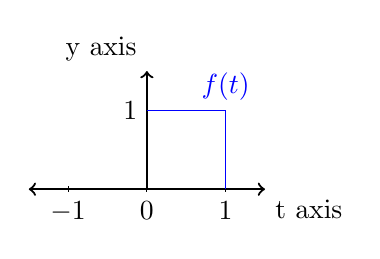
\begin{tikzpicture}
				\centering
				\draw[thick,<->] (-1.5,0) -- (1.5,0) node[anchor=north west] {t axis};
				\draw[thick,->] (0,0) -- (0,1.5) node[anchor=south east] {y axis};
				\foreach \x in {-1,0,1}
				\draw (\x cm,1pt) -- (\x cm,-1pt) node[anchor=north] {$\x$};
				\foreach \y in {1}
				\draw (0,\y cm) -- (0,\y cm) node[anchor=east] {$\y$};
				\draw[blue] (0,1) -- (1,1) node[anchor=south] {$f(t)$}-- (1,0) ;
			\end{tikzpicture}
		\end{center}
	\caption{Functie $f(t)$}
	\end{subfigure}%
	\begin{subfigure}{.4\textwidth}
		\begin{center}
					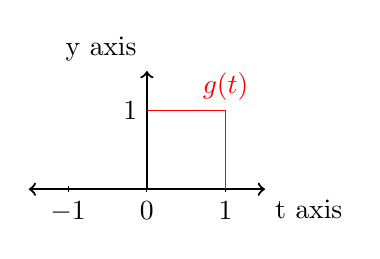
\begin{tikzpicture}
				\centering
				\draw[thick,<->] (-0.5,0) -- (2.5,0) node[anchor=north west] {t axis};
				\draw[thick,->] (1,0) -- (1,1.5) node[anchor=south east] {y axis};
				\foreach \x in {-1,0,1}
				\draw (\x cm +1cm,1pt) -- (\x cm+ 1 cm,-1pt) node[anchor=north] {$\x$};
				\foreach \y in {1}
				\draw (1,\y cm) -- (1,\y cm) node[anchor=east] {$\y$};
				\draw[red] (1,1) -- (2,1) node[anchor=south] {$g(t)$}-- (2,0) ;
			\end{tikzpicture}
		\end{center}
	\caption{Functie $g(t)$}
	\end{subfigure}
\caption{Te convolueren pulsen}
\label{fig:convoVoorbeeld}
\end{figure}
De functies in figuur \ref{fig:convoVoorbeeld} kunnen we wiskundig beschrijven als:
\begin{equation}
	f(t) = g(t) = u(t)-u(t-1)
\end{equation}
Als we hier de definitie op toepassen, zien we dat we de functie $g(t)$ moeten spiegelen tegenover de x as vanwege het minteken in het argument in vergelijking \ref{eq:defConvo}.  We krijgen dus volgende figuren: \\

\begin{figure}[h]
	\centering
	\begin{subfigure}{.4\textwidth}
		\begin{center}
			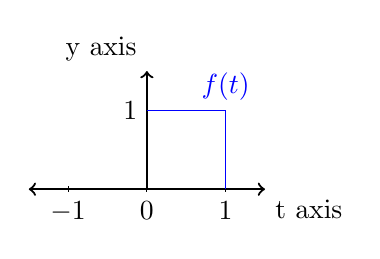
\begin{tikzpicture}
				\centering
				\draw[thick,<->] (-1.5,0) -- (1.5,0) node[anchor=north west] {t axis};
				\draw[thick,->] (0,0) -- (0,1.5) node[anchor=south east] {y axis};
				\foreach \x in {-1,0,1}
				\draw (\x cm,1pt) -- (\x cm,-1pt) node[anchor=north] {$\x$};
				\foreach \y in {1}
				\draw (0,\y cm) -- (0,\y cm) node[anchor=east] {$\y$};
				\draw[blue] (0,1) -- (1,1) node[anchor=south] {$f(t)$}-- (1,0) ;
			\end{tikzpicture}
		\end{center}
		\caption{Functie $f(t)$}
	\end{subfigure}%
	\begin{subfigure}{.4\textwidth}
		\begin{center}
			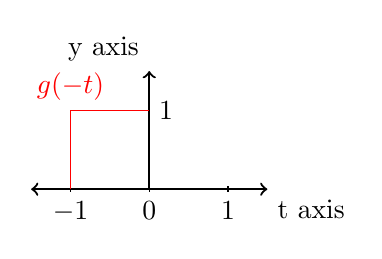
\begin{tikzpicture}
				\centering
				\draw[thick,<->] (-0.5,0) -- (2.5,0) node[anchor=north west] {t axis};
				\draw[thick,->] (1,0) -- (1,1.5) node[anchor=south east] {y axis};
				\foreach \x in {-1,0,1}
				\draw (\x cm +1cm,1pt) -- (\x cm+ 1 cm,-1pt) node[anchor=north] {$\x$};
				\foreach \y in {1}
				\draw (1,\y cm) -- (1,\y cm) node[anchor=west] {$\y$};
				\draw[red] (0,0) -- (0,1) node[anchor=south] {$g(-t)$}-- (1,1) ;
			\end{tikzpicture}
		\end{center}
		\caption{Functie $g(-t)$}
	\end{subfigure}
	\caption{Toepassing van de definitie}
	\label{fig:convoVoorbeeld2}
\end{figure}
Nu kunnen we de functie $g(-t)$ laten schuiven over de functie $f(t)$. Dit proces wordt weergegeven in figuur \ref{fig:convoSchuiven}. \\

\begin{figure}[h]
	\centering
	\begin{subfigure}{.4\textwidth}
		\begin{center}
			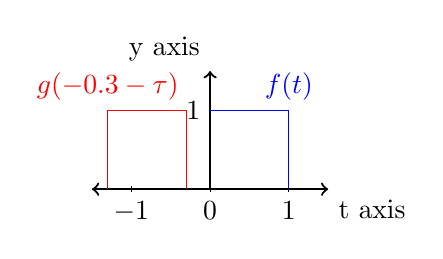
\begin{tikzpicture}
				\centering
				\draw[thick,<->] (-1.5,0) -- (1.5,0) node[anchor=north west] {t axis};
				\draw[thick,->] (0,0) -- (0,1.5) node[anchor=south east] {y axis};
				\foreach \x in {-1,0,1}
				\draw (\x cm,1pt) -- (\x cm,-1pt) node[anchor=north] {$\x$};
				\foreach \y in {1}
				\draw (0,\y cm) -- (0,\y cm) node[anchor=east] {$\y$};
				\draw[blue] (0,1) -- (1,1) node[anchor=south] {$f(t)$}-- (1,0) ;
				\draw[red] (-1.3,0) -- (-1.3,1) node[anchor=south] {$g(-0.3-\tau)$}-- (-0.3,1) -- (-0.3,0) ;
			\end{tikzpicture}
		\end{center}
		\caption{Functie $g(-0.3 -\tau)$}
	\end{subfigure}%
		\begin{subfigure}{.4\textwidth}
		\begin{center}
			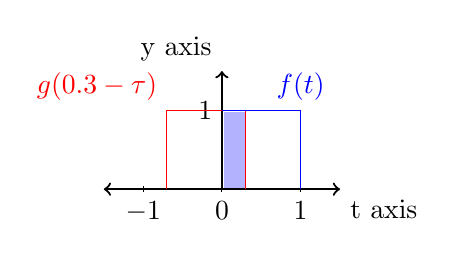
\begin{tikzpicture}
				\centering
				\draw[thick,<->] (-1.5,0) -- (1.5,0) node[anchor=north west] {t axis};
				\draw[thick,->] (0,0) -- (0,1.5) node[anchor=south east] {y axis};
				\foreach \x in {-1,0,1}
				\draw (\x cm,1pt) -- (\x cm,-1pt) node[anchor=north] {$\x$};
				\foreach \y in {1}
				\draw (0,\y cm) -- (0,\y cm) node[anchor=east] {$\y$};
				\draw[red] (-0.7,0) -- (-0.7,1) node[anchor=south east] {$g(0.3-\tau)$}-- (0.3,1) -- (0.3,0) ;
				\draw[blue] (0,1) -- (1,1) node[anchor=south] {$f(t)$}-- (1,0) ;
				\fill[blue!30!white] (0.02,0.02) rectangle (0.29,0.98);
			\end{tikzpicture}
		\end{center}
		\caption{Functie $g(0.3 -\tau)$}
	\end{subfigure}%
	\caption{Toepassing van de definitie}
	\label{fig:convoSchuiven}
\end{figure}
We laten dit proces door gaan tot de de functies volledig over elkaar geschoven zijn.  Dit is de visuele interpretatie van een convolutie
\newpage
Wiskundig kunnen we deze convolutie als volgt uitwerken:
\begin{align}
	(f\ast g)(t) &= \int_{-\infty}^{\infty} f(\tau) g(t-\tau) d\tau\\
	&= \int_{-\infty}^{\infty}\left[  u(t)-u(t-1)\right]  \cdot \left[ u(t)-u(t-1)\right] d\tau
\end{align}
We kunnen nu twee gevallen onderscheiden op basis van de waarde van $t$. Figuur \ref{fig:tweeGevallen} illustreert deze 2 gevallen. \\

\begin{figure}[h]
	\centering
	\begin{subfigure}{.4\textwidth}
		\begin{center}
			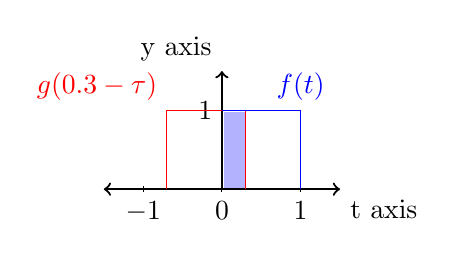
\begin{tikzpicture}
				\centering
				\draw[thick,<->] (-1.5,0) -- (1.5,0) node[anchor=north west] {t axis};
				\draw[thick,->] (0,0) -- (0,1.5) node[anchor=south east] {y axis};
				\foreach \x in {-1,0,1}
				\draw (\x cm,1pt) -- (\x cm,-1pt) node[anchor=north] {$\x$};
				\foreach \y in {1}
				\draw (0,\y cm) -- (0,\y cm) node[anchor=east] {$\y$};
				\draw[red] (-0.7,0) -- (-0.7,1) node[anchor=south east] {$g(0.3-\tau)$}-- (0.3,1) -- (0.3,0) ;
				\draw[blue] (0,1) -- (1,1) node[anchor=south] {$f(t)$}-- (1,0) ;
				\fill[blue!30!white] (0.02,0.02) rectangle (0.29,0.98);
			\end{tikzpicture}
		\end{center}
		\caption{ $t\leq 1$}
	\end{subfigure}%
	\begin{subfigure}{.4\textwidth}
		\begin{center}
			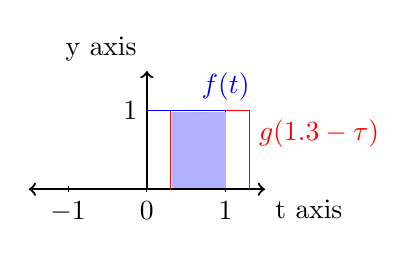
\begin{tikzpicture}
				\centering
				\draw[thick,<->] (-1.5,0) -- (1.5,0) node[anchor=north west] {t axis};
				\draw[thick,->] (0,0) -- (0,1.5) node[anchor=south east] {y axis};
				\foreach \x in {-1,0,1}
				\draw (\x cm,1pt) -- (\x cm,-1pt) node[anchor=north] {$\x$};
				\foreach \y in {1}
				\draw (0,\y cm) -- (0,\y cm) node[anchor=east] {$\y$};
				\draw[red] (0.3,0) -- (0.3,1) -- (1.3,1) node[anchor=north west] {$g(1.3-\tau)$}-- (1.3,0) ;
				\draw[blue] (0,1) -- (1,1) node[anchor=south] {$f(t)$}-- (1,0) ;
				\fill[blue!30!white] (0.32,0.02) rectangle (1,0.98);
			\end{tikzpicture}
		\end{center}
		\caption{$t\geq 1$}
	\end{subfigure}%
	\caption{twee gevallen}
	\label{fig:tweeGevallen}
\end{figure}
De conclusie die we hieruit kunnen trekken is dat we voor elk geval apart een eenvoudige integraal kunnen opstellen. 
\begin{align}
	(f\ast g)(t) &= \int_{0}^{t}1d\tau = t \quad&\text{voor}\quad 0\leq t\leq 1\\
	(f\ast g)(t) &= \int_{t-1}^{1}1d\tau = -t+2 \quad&\text{voor} \quad1\leq t\leq 2\\
	(f\ast g)(t) &= 0 \quad&\text{voor} \quad t\leq 0\vee t\geq 2
\end{align}
Grafisch kunnen we het resultaat van deze convolutie als volgt weergeven: 
\begin{center}
	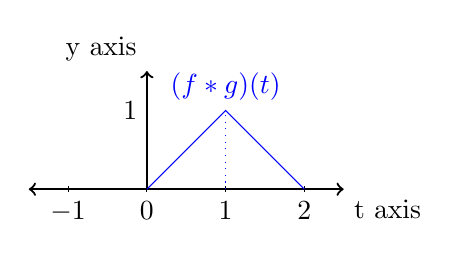
\begin{tikzpicture}
		\centering
		\draw[thick,<->] (-1.5,0) -- (2.5,0) node[anchor=north west] {t axis};
		\draw[thick,->] (0,0) -- (0,1.5) node[anchor=south east] {y axis};
		\foreach \x in {-1,0,1,2}
		\draw (\x cm,1pt) -- (\x cm,-1pt) node[anchor=north] {$\x$};
		\foreach \y in {1}
		\draw (0,\y cm) -- (0,\y cm) node[anchor=east] {$\y$};
		\draw[blue] (0,0) -- (1,1) node[anchor=south] {$(f\ast g)(t)$}-- (2,0) ;
		\draw[blue, dotted] (1,0) -- (1,1);
	\end{tikzpicture}
\end{center}
\end{document}
